

\section[Semantic Similarity]{Semantic Similarity }
\subsection{ }




\frame{
\frametitle{Similarity Measures }

\begin{itemize}
  \item \textbf{Similarity measure} is a numerical measure of the degree the two objects are alike  
  \item \textbf{Dissimilarity measure} is a numerical measure of the degree to which the two objects are different.
  \item Both similarity and dissimilarity scores are scalars in range $[0;1]$ or $[0;\infty]$.
  \item Two similar objects $i$ and $j$ will have a high similarity score $s_{ij}$ and a low dissimilarity score $d_{ij}$.
  \item Similarity to dissimilarity and vice versa:
 \begin{itemize}
    \item if $d_{ij} \in [0;1]$, then $s_{ij} = 1 -d_{ij}$, where $s_{ij} \in [0;1]$;
    \item if $s_{ij} \in [0;1]$, then $d_{ij} = 1 - s_{ij}$, where $d_{ij} \in [0;1]$;
    \item if $d_{ij} \in [0;\infty]$, then $s_{ij} = 1 - \frac{d_{ij} - \min_{i,j}(d_{ij})}{\max_{i,j}(d_{ij}) - \min_{i,j}(d_{ij}) }$, where $s_{ij} \in [0;1]$;
    \item if $s_{ij} \in [0;\infty]$, then $d_{ij} = 1 - \frac{s_{ij} - \min_{i,j}(s_{ij})}{\max_{i,j}(s_{ij}) - \min_{i,j}(s_{ij}) }$, where $d_{ij} \in [0;1]$.
\end{itemize}
\end{itemize} 

\textit{Definitions are adapted from (Tan, 2006).}


}



\begin{frame}
\frametitle{Semantic Similarity Measures}



\begin{block}{Definition}
  A semantic similarity measure quantifies semantic relatedness input terms $c_i, c_j$ with the similarity score $s_{ij} = sim(c_i,c_j)$:
    $$
  s_{ij} = \left\{ 
   \begin{array}{l l}
     1 & \quad \text{if } \langle c_i, c_j \rangle \text{ is a pair of } syn, hyper, cohypo \\
    0 & \quad \text{otherwise}\\
   \end{array} \right.
 $$
 \end{block}


\begin{block}{Properties}
\begin{itemize}    
  \item Nonnegativity: $0 \leq s_{ij} \leq 1$;
  \item Reflexivity: $s_{ij} = 1 \Leftrightarrow c_i = c_j$;
  \item Symmetricity: $s_{ij} = s_{ji}$;
  \end{itemize}
 \end{block}
     
\end{frame}



\frame{
\frametitle{Word similarity matrix $\mathbf{S}$}


\begin{itemize}
\item  $\mathbf{S}$ -- word $*$ word similarity matrix;
\item $s_{ij} \in \mathbf{S}$ -- similarity of words $w_i$ and $w_j$;
\item $s_{ij} = sim(w_i, w_j), s_{ij} \in [0;1].$
\end{itemize}

\begin{figure}
\centering
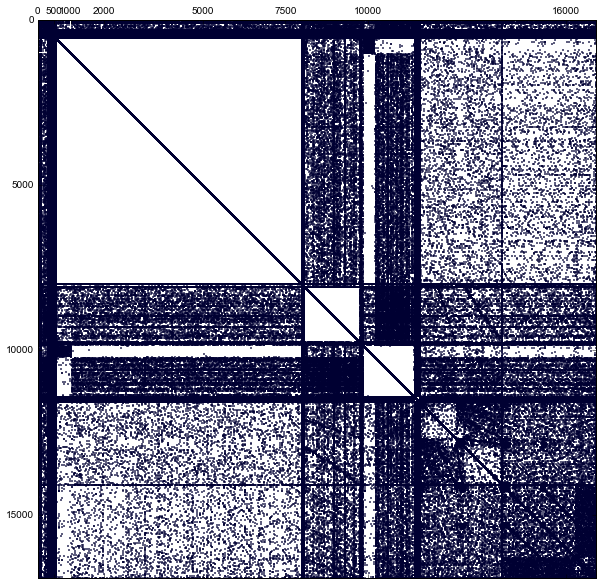
\includegraphics[width=0.5\textwidth]{./figures/simm}
\end{figure}

}




\begin{frame}
\frametitle{Semantic Similarity Measures}
\begin{itemize}

\item Many dissimilar pairs, few similar pairs: $s_{ij} \sim exp(\lambda)$:

\begin{figure}
\centering
\includegraphics[width=0.5\textwidth]{./../figures/reldist-crop}
\end{figure}

\item Similarity distribution of the term ``doctor'': 

\begin{figure}
\centering
\includegraphics[width=0.6\textwidth]{./../figures/real-extracted}
\end{figure} 

\end{itemize}
\end{frame}




\begin{frame}
\frametitle{Number of relations in semantic resources}
\begin{figure}
\centering
\includegraphics[width=0.9\textwidth]{./../figures/reldist}
\caption{ Number of relations (synonyms and hyponyms) per term in the dictionaries: a dictionary of synonyms, Roget's thesaurus, WordNet and a union of these three resources.  }
\label{fig:sim-distribution}
\end{figure}

\end{frame}


\begin{frame}
\frametitle{Evaluation of Semantic Similarity Measures}

\begin{enumerate}
\item correlations with human judgments (\textbf{MC}, \textbf{RG}, \textbf{WordSim});
\item semantic relation ranking (\textbf{BLESS}, \textbf{SN});
\item semantic relation extraction;
\item using extracted relations in an application:
\begin{itemize}
\item a short text classification system (\textbf{iCOP});
\item a lexico-semantic search engine (\textbf{Serelex}).
\end{itemize}
\end{enumerate}

\end{frame}









\begin{frame}
\frametitle{Evaluation of Semantic Similarity Measures}

\begin{enumerate}
\item \textbf{Correlations with human judgments}:
\begin{itemize}
 \item Criterion: Pearson correlation ($\rho$) О Spearman correlation ($r$).
 \item Datasets: MC, RG, WordSim.
\end{itemize}

\item \textbf{Semantic relation ranking}:
\begin{itemize}
 \item Criterion: Precision, Recall, F-measure.
 \item Dataset: BLESS, SN.
\end{itemize}


\item \textbf{Semantic relation extraction:}
\begin{itemize}
 \item Criterion: Precision@k.
 \item Data: annotation and/or dictionaries.
\end{itemize}

\item \textbf{Application-based evaluation:}
\begin{itemize}
\item short text classification system (\textbf{iCOP});
\item lexico-semantic search engine (\textbf{Serelex}).
\end{itemize}
\end{enumerate}


Panchenko A., \textbf{Similarity Measures for Semantic Relation Extraction.} PhD thesis. Universit\'{e} catholique de Louvain. 197 pages, 2013, (Chapter 1). 

\end{frame}







\begin{frame}
\frametitle{Correlations with human judgments}

\begin{table}[h]\footnotesize
\begin{tabular}{ |c|c|c|c|c|c| }
\hline
  word, $c_i$ & word, $c_j$ & human, $\mathbf{s}$  & sim, $\mathbf{s}$  & human (rank), $\mathbf{r}$ & sim (rank), $\hat{\mathbf{r}}$  \\ \hline \hline
tiger & cat & 7.35 & 0.85 & 1 & 3 \\
book & paper & 7.46 &  0.95 & 2 & 2 \\
computer & keyboard & 7.62 &  0.81 & 3 & 1 \\
... & ... & ... & ...   & \ldots & \ldots \\
possibility & girl & 1.94 & 0.25 & 64 & 65 \\
sugar & approach & 0.88 & 0.05 & 65 & 23 \\ \hline
\end{tabular}
\end{table}


\textbf{Datasets:}

\begin{itemize}
    \item WordSim353 -- 353 word pairs (Finkelstein, 2002)  
    \item MC -- 30 word pairs  (Miller & Charles, 1991)
    \item RG -- 65 word pairs (Rubenstein & Goodenough, 1965)  
\end{itemize}

\textbf{Pearson correlation:}  $\rho = \frac{cov(\mathbf{s},\hat{\mathbf{s}})}{\sigma(\mathbf{s}) \sigma(\hat{\mathbf{s}})}$

 \textbf{Spierman correlation:}: $r = \frac{cov(\mathbf{r},\hat{\mathbf{r}})}{\sigma(\mathbf{r}) \sigma(\hat{\mathbf{r}})}$
\end{frame}



\begin{frame}
\frametitle{Correlations with human judgments}

\begin{figure}
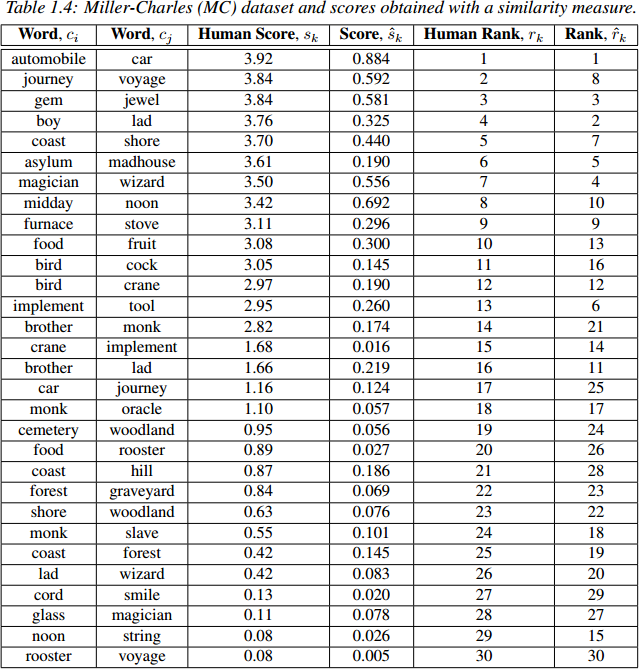
\includegraphics[height=0.6\textwidth]{./figures/rg}
\end{figure}


\end{frame}



\begin{frame}
\frametitle{Correlations with human judgments}

\begin{figure}
    \centering
        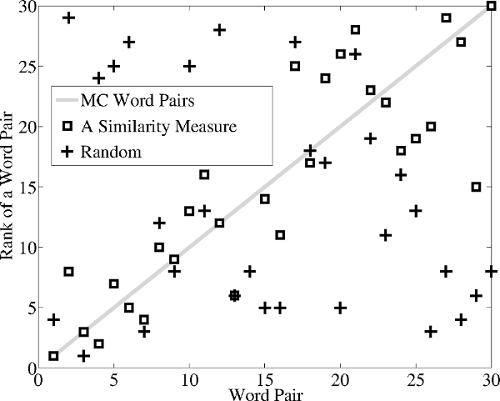
\includegraphics[width=0.55\textwidth]{../figures/mc-correlations-2}
    \caption{ Spearman correlation on the Miller-Charles (MC) dataset. $\rho$ of a similarity measure is 0.843 (p<0.001) and $\rho$ of a random measure is -0.173 (p=0.360). }
    \label{fig:mc-correlations}
\end{figure}
\end{frame}



%%%%%%%%%%%%%%%%%%%%%%%%%%%%%%%%%%%%%%%%%%%%%%%%%



%%%%%%%%%%%%%%%%%%%%%%%%%%%%%%%%%%%%%%%%%%%%%%%%%
\begin{frame}
\frametitle{Semantic Relation Ranking and Classification}

{ \scriptsize

\begin{table}[h]\footnotesize
\begin{tabular}{ |c|l|l| }
\hline
\bf слово, $c_i$ & \bf  слово, $c_j$ & \bf тип отношения, $t$  \\ \hline \hline
judge & adjudicate & syn \\
judge & arbitrate & syn \\
judge & asessor & syn \\
... & ... & ...   \\
judge & pc & random \\ 
judge & fare & random \\
judge & lemon & random \\ \hline
\end{tabular}
\end {table}

}

\textbf{Datasets:}
\begin{itemize}
  \item BLESS (Baroni and Lenci, 2011)  -- 26554 relations (hyper, coord, mero, event, attri, random)  
  \item SN (Panchenko, 2012) -- 14682  relations (syn, random) 
 \item RT, AE, AE2 (Panchenko et al., 2015)

\end{itemize}

\end{frame}



\begin{frame}
\frametitle{Semantic Relation Ranking  and Classification}

\begin{itemize}
   \item Precision $P(k=50)= \frac{1}{7} \approx 0.86 $
\end{itemize}


\begin{table}[h]\footnotesize
\begin{tabular}{ |l|l|l|l| }
\hline
\bf word, $c_i$ & \bf  word, $c_j$ & \bf relation type & \bf $s_{ij}$ \\ \hline \hline

aficionado & enthusiast & syn & 0.07197 \\
aficionado & fan & syn & 0.05195 \\
aficionado & admirer & syn & 0.01964 \\
aficionado & addict & syn & 0.01326 \\
aficionado & devotee & syn & 0.01163 \\
\alert{aficionado} & \alert{foundling} & \alert{random} & \alert{0.00777} \\
aficionado & fanatic & syn & 0.00414 \\ \hline
aficionado & adherent & syn & 0.00353 \\
aficionado & capital & random & 0.00232 \\
aficionado & statute & random & 0.00029 \\
aficionado & blot & random & 0.00025 \\
aficionado & meddler & random & 0.00005 \\
aficionado & enlargement & random & 0.00003 \\
aficionado & bawdyhouse & random &  0.00000 \\ 
\hline
\end{tabular}
\end {table}

\end{frame}



\begin{frame}
\frametitle{Semantic Relation Ranking  and Classification: BLESS}

\begin{table*}
\centering
%\caption{A target word ``hawk" and all its relatum words from the BLESS dataset ranked by similarity score. The table on the left      contains relations retrieved with the $k$-NN threshold of 50$\%$ The whole table contains all relations of the word ($k=100\%). }
\includegraphics[width=0.55\textwidth]{../figures/bless-example}
\label{tbl:bless-example}
\end{table*}
    
\end{frame}


%%%%%%%%%%%%%%%%%%%%%%%%%%%%%%%%%%%%%%%%%%%%%%%%%
\begin{frame}
\frametitle{Semantic Relation Ranking  and Classification}

\begin{itemize}
  
  \item Based on the number of  \alert{correctly classified or ranked} semantic relations.
  

\item $R$ -- set of non-random relations, e.g. not like $\langle animal, random, bishop \rangle$

\item $\hat{R}(k)$ set of extracted relations at $k$ nearest neighbours

\begin{block}{Evaluation metrics}

    
    \begin{itemize}
        \item Precision: $P(k)=$$\frac{|R \cap \hat{R}(k)|}{|\hat{R}(k)|}$,
        \item Recall: $R(k)=$$\frac{|R \cap \hat{R}(k)|}{|R|}$,
        \item F1-measure: $F(k)= 2 \cdot \frac{P(k) \cdot R(k)}{P(k) + R(k)}$,
    \end{itemize}   
    \end{block}

    

\end{itemize}
    
\end{frame}



